%% LyX 2.3.6.1 created this file.  For more info, see http://www.lyx.org/.
%% Do not edit unless you really know what you are doing.
\documentclass[english]{article}
\usepackage[T1]{fontenc}
\usepackage[latin9]{inputenc}
\usepackage{geometry}
\geometry{verbose,tmargin=2.5cm,bmargin=2.5cm,lmargin=2.5cm,rmargin=2.5cm}
\usepackage{array}
\usepackage{textcomp}
\usepackage{multirow}
\usepackage{graphicx}

\makeatletter

%%%%%%%%%%%%%%%%%%%%%%%%%%%%%% LyX specific LaTeX commands.
%% Because html converters don't know tabularnewline
\providecommand{\tabularnewline}{\\}

\makeatother

\usepackage{babel}
\begin{document}
{[}SPLIT\_HERE{]}
\begin{enumerate}
\item \textbf{{[}NYJC/PRELIM/9569/2021/P1/Q1{]} }
\begin{enumerate}
\item The TCP/IP networking model comprises 4 layers. 
\begin{enumerate}
\item Copy and complete the below diagram for the TCP/IP stack.
\noindent \begin{center}
\begin{tabular}{|c|}
\hline 
\tabularnewline
\hline 
Transport Layer\tabularnewline
\hline 
\tabularnewline
\hline 
\tabularnewline
\hline 
\end{tabular}
\par\end{center}

\hfill{}{[}3{]}
\item State the purpose of the Transport Layer in the TCP/IP network model.
\hfill{}{[}2{]}
\item State the reserved port range used in the Transport Layer. \hfill{}{[}1{]}
\end{enumerate}
\item A certain port number in binary form is \texttt{00000100} \texttt{00011000}. 
\begin{enumerate}
\item Express this value in denary (decimal) form. \hfill{}{[}3{]}
\item Explain how it may be checked if this binary port value is within
the reserved port range, without converting it to decimal.\hfill{}{[}2{]}
\end{enumerate}
\item {}
\begin{enumerate}
\item State which layer of the TCP/IP model the Domain Name System (DNS)
protocol belongs to.\hfill{} {[}1{]}
\item Describe the purpose of the DNS protocol. \hfill{}{[}2{]}
\end{enumerate}
\end{enumerate}
{[}SPLIT\_HERE{]}
\item \textbf{{[}NYJC/PRELIM/9569/2021/P1/Q2{]} }
\begin{enumerate}
\item Validation and verification are used in data entry. 
\begin{enumerate}
\item State the purpose of validation. \hfill{}{[}1{]}
\item State the purpose of verification. \hfill{}{[}1{]}
\end{enumerate}
\end{enumerate}
A network program using TCP needs to check if a port number is within
an acceptable range of values.
\begin{enumerate}
\item[(b)]  Is this fulfilled by validation or verification? Explain your answer.\hfill{}
{[}2{]}
\item[(c)]  Provide three sets of suitable test values for the above check.
\hfill{}{[}3{]}
\end{enumerate}
{[}SPLIT\_HERE{]}
\item \textbf{{[}NYJC/PRELIM/9569/2021/P1/Q3{]} }

A printing shop needs to set up a print queue system to serve its
customers. This print queue will manage print tasks, by sending them
one at a time to available printers.

For all print tasks, the data that will be stored include: 

\noindent %
\noindent\begin{minipage}[t]{1\columnwidth}%
\texttt{\qquad{}}User 

\texttt{\qquad{}}Printer address 

\texttt{\qquad{}}Job name 

\texttt{\qquad{}}Status %
\end{minipage}

The print queue itself stores the following data: 

\texttt{\qquad{}}Number of jobs 

When a print task is added to the queue: 
\begin{itemize}
\item The task is stored inside the queue, in FIFO order 
\item The jobs count is incremented by one 
\end{itemize}
When a print task is sent to a printer: 
\begin{itemize}
\item The print task is removed from the queue, in FIFO order 
\item The jobs count is decremented by one
\end{itemize}
\begin{enumerate}
\item {}
\begin{enumerate}
\item Draw a class diagram that shows the following for the situation described
above. 
\begin{itemize}
\item The classes 
\item properties 
\item appropriate methods \hfill{}{[}9{]}
\end{itemize}
\item Explain the meaning of the terms: 
\begin{enumerate}
\item[1.]  inheritance \hfill{}{[}2{]}
\item[2.]  polymorphism \hfill{}{[}2{]}
\end{enumerate}
\end{enumerate}
\end{enumerate}
The printing shop wishes to implement a circular queue to limit the
maximum number of pending jobs and improve the performance of their
system. 
\begin{enumerate}
\item[(b)]  {}
\begin{enumerate}
\item State two differences between a linear queue and a circular queue.
\hfill{}{[}2{]}
\item Suggest whether inheritance or polymorphism is a more suitable principle
to apply in the implementation of both linear queue and circular queue
in the same program. Explain your answer. \hfill{}{[}4{]}
\end{enumerate}
\item[(c)]  Using a suitable diagram, pseudocode, or other method, show how
an item would be added to a circular queue implemented with a static
array. \hfill{}{[}4{]}
\end{enumerate}
{[}SPLIT\_HERE{]}
\item \textbf{{[}NYJC/PRELIM/9569/2021/P1/Q4{]} }

An algorithm for sorting an array of elements is shown. 

\noindent %
\noindent\begin{minipage}[t]{1\columnwidth}%
\texttt{01 FOR i = 1 to Array.LENGTH - 1 }

\texttt{02 \qquad{}FOR j = 1 to Array.LENGTH - 1 }

\texttt{03 \qquad{}\qquad{}IF Array{[}j{]} > Array{[}j+1{]} }

\texttt{04 \qquad{}\qquad{}\qquad{}THEN }

\texttt{05 \qquad{}\qquad{}\qquad{}\qquad{}t = Array{[}j{]} }

\texttt{06 \qquad{}\qquad{}\qquad{}\qquad{}Array{[}j{]} = Array{[}j+1{]} }

\texttt{07 \qquad{}\qquad{}\qquad{}\qquad{}Array{[}j+1{]} = t }

\texttt{08 \qquad{}\qquad{}ENDIF }

\texttt{09 \qquad{}ENDFOR }

\texttt{10 ENDFOR }%
\end{minipage}
\begin{enumerate}
\item {} 
\begin{enumerate}
\item State the algorithm represented. \hfill{}{[}1{]}
\item tate the time complexity of this algorithm. \hfill{}{[}1{]}
\item Copy and complete the trace table below with the value of \texttt{Array}
at the end of each iteration of \texttt{i} in the algorithm. \hfill{}{[}5{]}
\end{enumerate}
\noindent \begin{center}
\begin{tabular}{|c|c|}
\hline 
\texttt{i} & \texttt{Array}\tabularnewline
\hline 
Initial  & {[}2, 3, 4, 5, 6, 1{]}\tabularnewline
\hline 
1 & \tabularnewline
\hline 
2 & \tabularnewline
\hline 
3 & \tabularnewline
\hline 
4 & \tabularnewline
\hline 
5 & \tabularnewline
\hline 
6 & \tabularnewline
\hline 
\end{tabular}
\par\end{center}
\item Describe \textbf{two} improvements that could be made to the above
algorithm to improve its efficiency. \hfill{}{[}4{]}
\item Explain why insertion sort is usually used instead of bubble sort,
although both have the same time efficiency.\hfill{} {[}2{]}
\end{enumerate}
\item \textbf{{[}NYJC/PRELIM/9569/2021/P1/Q5{]} }

A school database has some data in the following table: 
\noindent \begin{center}
\begin{tabular}{|c|c|c|c|}
\hline 
\textbf{StudentID} & \textbf{Student Name } & \textbf{Class } & \textbf{Subjects}\tabularnewline
\hline 
1  & Wong Yong Ming  & 1917  & H2MATH, H2PHY, H2CHEM, H2ECON\tabularnewline
\hline 
2  & Vikram Singh  & 1911  & H2MATH, H2CHEM, H2ECON,H1GEOG\tabularnewline
\hline 
3  & Muhd Bashir bin Ramdan  & 1911 & H2MATH, H2CHEM, H2ECON, H1ELIT\tabularnewline
\hline 
\end{tabular} 
\par\end{center}
\begin{enumerate}
\item {}
\begin{enumerate}
\item State and explain if the above table is in third normal form (3NF).
\hfill{}{[}4{]}
\item Describe two advantages that normalised data has over redundant data.
\hfill{}{[}2{]}
\end{enumerate}
\end{enumerate}
In an effort to improve the school database, the IT administrator
came up with an ER diagram. Part of the full ER diagram is as shown. 
\begin{center}
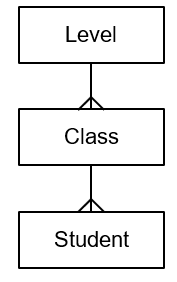
\includegraphics[width=0.15\paperwidth]{C:/Users/Admin/Desktop/Github/question_bank/LyX/static/img/9569-NYJC-2021-P1-Q5}
\par\end{center}

Each of the three entities in the ER diagram has a name attribute. 
\begin{enumerate}
\item[(b)] {}  
\begin{enumerate}
\item Write table descriptions to implement the above ER diagram. \hfill{}{[}5{]}
\item Write an SQL query to retrieve only the student name and class name
for all students in the level \texttt{JC2}. \hfill{}{[}3{]}
\end{enumerate}
\end{enumerate}
A fast-growing startup is writing code to provide a new service. The
user needs have not yet been fully determined, and the data schema
is likely to undergo further changes before being finalised. 
\begin{enumerate}
\item[(c)]  {}
\begin{enumerate}
\item Suggest if SQL or NoSQL is more suitable for the needs of this startup.
Give \textbf{two} reasons to support your answer.\hfill{} {[}4{]}
\item Describe \textbf{two} challenges the startup will face in using NoSQL
databases.\hfill{} {[}2{]}
\end{enumerate}
\item[(d)]  The startup is concerned that a hardware failure may wipe out critical
data and leave them unable to continue operating. 

Suggest what the startup should do to \textbf{ensure} that they are
safe against data loss in such a scenario.\hfill{} {[}4{]}
\end{enumerate}
{[}SPLIT\_HERE{]}
\item \textbf{{[}NYJC/PRELIM/9569/2021/P1/Q6{]} }

Alice, a programmer, is implementing a DNS cache using a hash table. 
\begin{enumerate}
\item Explain the purpose of the hash function in a hash table. \hfill{}
{[}2{]}
\end{enumerate}
The description for a particular hashing algorithm using rolling polynomials
is as follows: 

\noindent %
\noindent\begin{minipage}[t]{1\columnwidth}%
For each character in the data, do the following: 
\begin{enumerate}
\item[1]  Let \texttt{i} represent the position of the character (1st char
= 1, 2nd char = 2, ...) 
\item[2]  Let \texttt{ascii} represent the ASCII value of the character 
\item[3]  Calculate the sum of \texttt{i}\texttimes (31\textasciicircum\texttt{ascii})
for all characters 
\end{enumerate}
%
\end{minipage}
\begin{enumerate}
\item[(b)]  Implement this algorithm in pseudocode. 

You may assume that the function \texttt{Ord()} is available, which
takes in a single character and returns the ASCII value of the character.
\hfill{} {[}4{]}
\item[(c)]  Bob, another programmer, suggests that a Binary Search Tree would
be a more appropriate data structure for the DNS cache. 
\begin{enumerate}
\item Describe one advantage of using a hash table for the DNS cache.\hfill{}
{[}2{]}
\item Describe one advantage of using a Binary Search Tree for the DNS cache.\hfill{}
{[}2{]}
\end{enumerate}
\item[(d)]  {}
\begin{enumerate}
\item State the algorithm used to retrieve the sorted contents of a cache
from a Binary Search Tree.\hfill{} {[}1{]}
\item Using any appropriate diagrams, pseudocode, or other appropriate method,
show how this algorithm might be carried out. \hfill{} {[}5{]}
\item Explain why the Binary Search Tree might need to be periodically recreated.\hfill{}
{[}3{]}
\end{enumerate}
\end{enumerate}
{[}SPLIT\_HERE{]}
\item \textbf{{[}NYJC/PRELIM/9569/2021/P2/Q1{]} }

Name your Jupyter Notebook as 

\texttt{TASK1\_<your name>\_<centre number>\_<index number>.ipynb }

A text file, \texttt{TIDES.TXT}, contains the low and high tide information
for a coastal location for each day of a month. Each line contains
tab-delimited data that shows the date, the time, whether the tide
is high or low and the tide height in metres. 

Each line is in the format: 

\texttt{YYYY-MM-DD\textbackslash tHH:mm\textbackslash tTIDE\textbackslash tHEIGHT\textbackslash n }
\begin{itemize}
\item The date is in the form YYYY-MM-DD, for example, 2019-08-03 is 3rd
August, 2019 
\item The time is in the form HH:mm, for example, 13:47 
\item TIDE is either HIGH or LOW 
\item HEIGHT is a positive number shown to one decimal place 
\item \texttt{\textbackslash t} represents the tab character 
\item \texttt{\textbackslash n} represents the newline character 
\end{itemize}
The text file is stored in ascending order of date and time. 

For each of the sub-tasks, add a comment statement, at the beginning
of the code using the hash symbol \textquoteleft \#\textquoteright ,
to indicate the sub-task the program code belongs to, for example: 
\noindent \begin{center}
\begin{tabular}{c|l|}
\cline{2-2} 
\multirow{2}{*}{\texttt{In{[}1{]}:}} & \texttt{\# Task 1.1}\tabularnewline
 & \texttt{Program Code}\tabularnewline
\cline{2-2} 
\multicolumn{1}{c}{} & \multicolumn{1}{l}{\texttt{Output:}}\tabularnewline
\end{tabular}
\par\end{center}

\subsubsection*{Task 1.1 }

Write program code to: 
\begin{itemize}
\item read the tide data from a text file 
\item find the highest high tide and print this value 
\item find the lowest low tide and print this value 
\end{itemize}
Use \texttt{TIDES.TXT} to test your program code.\hfill{} {[}7{]}

Save your Jupyter Notebook for Task 1. 

\subsubsection*{Task 1.2 }

The tidal range is the difference between the heights of successive
tides; from a high tide to the following low tide or from a low tide
to the following high tide. 

Amend your program code to: 
\begin{itemize}
\item output the largest tidal range and the date on which the second tide
occurs 
\item output the smallest tidal range and the date on which the second tide
occurs 
\end{itemize}
Use \texttt{TIDES.TXT} to test your program code. \hfill{}{[}4{]}

{[}SPLIT\_HERE{]}
\item \textbf{{[}NYJC/PRELIM/9569/2021/P2/Q2{]} }

Name your Jupyter Notebook as 

\texttt{TASK2\_<your name>\_<centre number>\_<index number>.ipynb }

The task is to implement a todo list using a linkedlist data structure.
For each of the sub-tasks, add a comment statement, at the beginning
of the code using the hash symbol \textquoteleft \texttt{\#}\textquoteright ,
to indicate the sub-task the program code belongs to, for example: 
\noindent \begin{center}
\begin{tabular}{c|l|}
\cline{2-2} 
\multirow{2}{*}{\texttt{In{[}1{]}:}} & \texttt{\# Task 2.1}\tabularnewline
 & \texttt{Program Code}\tabularnewline
\cline{2-2} 
\multicolumn{1}{c}{} & \multicolumn{1}{l}{\texttt{Output:}}\tabularnewline
\end{tabular}
\par\end{center}

\subsubsection*{Task 2.1 }

The class \texttt{TodoList} represents a LinkedList and has the following
attributes: 
\begin{itemize}
\item \texttt{\_\_head} -- a pointer to the first node of the LinkedList;
if empty, it has a value of \texttt{None} 
\item \texttt{\_\_tail} -- a pointer to the last node of the LinkedList;
if empty, it has a value of \texttt{None} 
\end{itemize}
\texttt{TodoList} has the following methods defined on it: 
\begin{itemize}
\item \texttt{add(item)} -- wraps \texttt{item} in a \texttt{TodoItem}
instance, and adds it to the end of the LinkedList 
\item \texttt{remove(item)} -- removes the first \texttt{TodoItem} containing
\texttt{item} from the LinkedList 
\item \texttt{list()} -- returns a Python list containing each \texttt{item}
in the TodoList 
\end{itemize}
The class \texttt{TodoItem} represents a Node of the LinkedList and
has the following attributes: 
\begin{itemize}
\item \texttt{title} -- a short description of the todo item 
\item \texttt{\_\_next} -- a pointer to the next node in the LinkedList;
if this is the last node, it has a value of None 
\end{itemize}
\texttt{TodoItem} has the following methods defined on it: 
\begin{itemize}
\item l\texttt{ink\_to(todoitem)} -- links this \texttt{TodoItem} instance
to \texttt{todoitem}, another instance of the TodoItem class 
\end{itemize}
Implement the above classes. \hfill{}{[}13{]}

\subsubsection*{Task 2.2 }

Add the following items to a new \texttt{TodoList}: 
\begin{itemize}
\item \textquotedblleft Buy milk\textquotedblright{} 
\item \textquotedblleft Buy flour\textquotedblright{} 
\item \textquotedblleft Buy eggs\textquotedblright{}
\item \textquotedblleft Bake cake\textquotedblright{} 
\end{itemize}
Display the contents of the \texttt{TodoList}. \hfill{}{[}7{]}

\subsubsection*{Task 2.3 }

Remove the following items from the \texttt{TodoList}: 
\begin{itemize}
\item \textquotedblleft Buy milk\textquotedblright{} 
\item \textquotedblleft Buy eggs\textquotedblright{} 
\end{itemize}
Display the contents of the \texttt{TodoList}. \hfill{}{[}3{]}

Save your Jupyter Notebook for Task 2. 

{[}SPLIT\_HERE{]}
\item \textbf{{[}NYJC/PRELIM/9569/2021/P2/Q3{]} }

Name your Jupyter Notebook as 

\texttt{TASK3\_<your name>\_<centre number>\_<index number>.ipynb }

The task is to write a function that takes a sequence of characters
representing a colour, and translates the colour into a different
number base. 

8-bit colours are represented with three numbers, indicating the level
of the colours red (R), green (G), and blue (B) respectively. Each
number is an integer from 0 to 255. 255 represents the fully saturated
colour, while 0 represents zero saturation (black).

In HTML, these colours may be represented using hex code as well.
In hex code, the R, G, and B values are converted to hexadecimal.
Hex codes begin with the symbol \textquoteleft \#\textquoteright{}
followed by the three R, G, and B hexadecimal values. 

For example, the hex code \#0A0B0C represents a colour with RGB values
10, 11, and 12 respectively. 

For each of the sub-tasks, add a comment statement, at the beginning
of the code using the hash symbol \textquoteleft \#\textquoteright ,
to indicate the sub-task the program code belongs to, for example: 
\noindent \begin{center}
\begin{tabular}{c|l|}
\cline{2-2} 
\multirow{2}{*}{\texttt{In{[}1{]}:}} & \texttt{\# Task 3.1}\tabularnewline
 & \texttt{Program Code}\tabularnewline
\cline{2-2} 
\multicolumn{1}{c}{} & \multicolumn{1}{l}{\texttt{Output:}}\tabularnewline
\end{tabular}
\par\end{center}

\subsubsection*{Task 3.1 }

Write a function called \texttt{task3\_1(hex)} that: 
\begin{itemize}
\item takes \texttt{hex}, a string representing a hex code, beginning with
a \textquoteleft \#\textquoteright{} symbol followed by three valid
hexadecimal values between 00 and FF 
\item returns and displays either: 
\begin{itemize}
\item a 3-integer tuple representing RGB values 

or 
\item the error message, \textquotedbl\texttt{invalid data}\textquotedbl{}
\hfill{}{[}5{]}
\end{itemize}
\end{itemize}
Test the function fully with suitable test data. 

For example, 

\texttt{task3\_1(\textquotedbl\#FFFFFF\textquotedbl ) }

should return and display \texttt{(255, 255, 255)}\hfill{} {[}3{]}

\subsubsection*{Task 3.2 }

Some image programs do not represent colours using 8-bit integers.
Instead, they represent them as a normalised float value. In this
representation, a value of 1.0 represents the fully saturated colour
and a value of 0 represents zero saturation (black). 

Write a second function \texttt{task3\_2(rgb)} that: 
\begin{itemize}
\item takes a 3-integer tuple rgb representing RGB values 
\item returns and displays either: 
\begin{itemize}
\item a 3-float tuple representing normalised RGB 

or 
\item the error message, \textquotedbl invalid data\textquotedbl{} \hfill{}{[}5{]}
\end{itemize}
\end{itemize}
Test the function fully with suitable test data. 

For example, 

\texttt{task3\_2((128, 128, 128))} 

should return and display\texttt{ (0.50196, 0.50196, 0.50196) }

\texttt{task3\_2((255, 255, 255)) }

should return and display\texttt{ (1.0, 1.0, 1.0)}\hfill{} {[}3{]}

\subsubsection*{Task 3.3 }

Image filters are functions that take in image data and change the
RGB values of its colours according to an algorithm. The algorithm
for converting an image to grayscale calculates the average of the
RGB values and sets the R, G, and B values to this average. 

Write a third function \texttt{task3\_3(hex)} that:
\begin{itemize}
\item takes hex, a string representing a hex code 
\item returns and displays a 3-float tuple representing normalised RGB of
the colour converted to grayscale \hfill{}{[}4{]}
\end{itemize}
Test the function fully with \textbf{two} suitable values.

For example, 

\texttt{task3\_3(\textquotedbl\#FF8000\textquotedbl ) }

should return and display \texttt{(0.5, 0.5, 0.5)}\hfill{} {[}2{]}

Save your Jupyter Notebook for Task 3.

{[}SPLIT\_HERE{]}
\item \textbf{{[}NYJC/PRELIM/9569/2021/P2/Q4{]} }

A bookstore uses a text file to store data about its inventory of
books. The bookshop carries two kinds of books: printed books and
virtual books. The bookshop wishes to transfer this information into
a database. 

The bookshop also wishes to create an online bookstore that allows
users to add books to a shopping cart for purchase.

\subsubsection*{Task 4.1}

Create an SQL file called \texttt{TASK4\_1\_<centre number>\_<index
number>.sql} to show the SQL code to create database \texttt{bookstore.db}
with three tables: \texttt{Book}, \texttt{Printed}, and \texttt{Virtual}.
The Printed and Virtual tables represent physical and virtual books
respectively, and stores properties unique to each type of book. 

The \texttt{Book} table will have the following fields: 
\begin{itemize}
\item \texttt{BookID} -- the primary key, an integer value 
\item \texttt{Title} -- the title of the book 
\item \texttt{Price} -- the price of the book, in cents 
\item \texttt{Type} -- the type of book: \textquotedbl physical\textquotedbl{}
or \textquotedbl virtual\textquotedbl{} 
\end{itemize}
The \texttt{Printed} table will have the following additional field: 
\begin{itemize}
\item \texttt{Weight} -- the weight of the book 
\end{itemize}
The \texttt{Virtual} table will have the following additional field: 
\begin{itemize}
\item \texttt{DownloadLink} -- the download link for the book 
\end{itemize}
Save your SQL code as 

\texttt{TASK4\_1\_<your name>\_<centre number>\_<index number>.sql}
\hfill{}{[}6{]}

\subsubsection*{Task 4.2 }

Python programming language and object-oriented programming will be
used to implement the online bookstore and shopping cart on a web
page. 

The class \texttt{Book} will store the following data: 
\begin{itemize}
\item \texttt{title} -- stored as a string 
\item \texttt{price} -- stored as an integer 
\end{itemize}
The class \texttt{Cart} will store the following data: 
\begin{itemize}
\item \texttt{items} -- stored as a list of \texttt{Book} objects 
\end{itemize}
The class \texttt{Cart} has a method defined on it: 
\begin{itemize}
\item \texttt{total\_price()} -- returns an integer representing the total
price of books in the cart 
\end{itemize}
Save your program code as 

\texttt{TASK4\_2\_<your name>\_<centre number>\_<index number>.py}
\hfill{}{[}6{]}

The \texttt{PrintedBook} class inherits from \texttt{Book}, and stores
the following additional data: 
\begin{itemize}
\item weight -- stored as an integer 
\end{itemize}
\texttt{Virtu}alBook class inherits from \texttt{Bo}ok, and stores
the following additional data: 
\begin{itemize}
\item download\_link -- stored as a string 
\end{itemize}
Add your program code to 

\texttt{TASK4\_2\_<your name>\_<centre number>\_<index number>.py}
{[}3{]} 

The text file, \texttt{bookstore.txt}, contains data items for books
stocked by the bookstore. Each data item is separated by a comma,
with each book\textquoteright s data on a new line as follows: 
\begin{itemize}
\item book title 
\item price 
\item type 
\item weight 
\item download link 
\end{itemize}
Write program code to read in the information from the text file,
\texttt{bookstore.txt}, creating an instance of the appropriate class
for each book (either \texttt{PrintedBook} or \texttt{VirtualBook}).
\hfill{}{[}4{]}

Write program code to insert all information from the file into the
\texttt{bookstore.db} database.

Run the program. Add your program code to 

\texttt{TASK4\_2\_<your name>\_<centre number>\_<index number>.py}
\hfill{}{[}8{]}

\subsubsection*{Task 4.3 }

The data from the text file, \texttt{bookstore.txt}, is to be used
to implement a shopping cart in a web browser. 

Write a Python program and the necessary files to create a web application
that: 
\begin{itemize}
\item displays a list of books stocked by the bookstore 
\item enables the user to add books to a shopping cart using an ID 
\item displays the contents of the shopping cart
\item shows the total price of items in the shopping cart 
\end{itemize}
For each book displayed the web page should include the: 
\begin{itemize}
\item book ID 
\item book title 
\item price 
\end{itemize}
Save your program as 

\texttt{TASK4\_3\_<your name>\_<centre number>\_<index number>.py }

with any additional files / sub-folders as needed in a folder named 

\texttt{TASK4\_3\_<your name>\_<centre number>\_<index number>}\hfill{}
{[}7{]}

Run the web application and add the following books to the shopping
cart: 
\begin{itemize}
\item Title: \textquotedbl Northanger Abbey\textquotedbl , Price: 13.99,
Type: Physical, Weight: 178g 
\item Title: \textquotedbl War and Peace\textquotedbl , Price: 17.49,
Type: Physical, Weight: 432g 
\item Title: \textquotedbl Computer Programs\textquotedbl , Price: 20.99,
Type: Virtual, Link: https://mybookstore.com/dJHtFy 
\item Title: \textquotedbl Data Science\textquotedbl , Price: 14.99, Type:
Virtual, Link: https://mybookstore.com/fJynJk 
\end{itemize}
Save the output of the program as

\texttt{TASK4\_3\_<your name>\_<centre number>\_<index number>.html}
\hfill{}{[}4{]}

{[}SPLIT\_HERE{]}
\end{enumerate}
 
\end{document}
